\chapter{Offre}
\section{Métier}
  %description du métier
\K{} est une société de conception et de création de
logiciels spécialisés dans le \gHabitat{}. Nous créons
ou améliorons des concepts existants en utilisant nos compétences
pour apporter une nouvelle expérience utilisateur. Ainsi, nous amenons
un plus grand confort d'utilisation aux professions du secteur en
leur fournissant des logiciels de qualité, autant au niveau du rendu
\mbox{final} (précision des calculs, lisibilité des rapports par des
professionnels ou des particuliers), qu'au niveau de l'utilisation
et de la rapidité de la saisie des informations
(DAO\footnote{\textbf{D}essin \textbf{A}ssité par \textbf{O}rdinateur} des plans,
interfaces de saisie ergonomique, superposition de calques).
\section{Valeur pour le client}
  %valeur pour le client
Notre société distribuera ses logiciel gratuitement ce qui permettra non
seulement aux petites structures (PME, TPE, professions libérales)
d'acquérir un logiciel qui améliorera leur productivité
au quotidien sans pour autant que cela représente un gros investissement 
entrainant souvent un emprunt,
mais également de permettre aux particuliers de faire des dimensionnements
thermiques normalisés de qualité sans avoir à passer par un bureau d'étude
pour peu qu'ils aient les connaissances nécessaires.

De plus nous apportons un gain d'ergonomie et une plus grande intuitivité
en intégrant des modules de saisie pour toutes les caractéristiques du bâtiment 
(bâtiment, zone, pièce, paroi, composant des parois) ainsi qu'une interface DAO
permettant de saisir directement le plan et les côtes des murs. Cette interface
graphique de saisie des plans facilite également la délimitation des différentes zone,
l'orientation du bâtiment ou encore de visualiser plusieurs étage simultanément grâce
à un système de clalques superposables.
\section{Produit}
  %présentation du produit
  \K{} travaille actuellement sur le developpement d'un logiciel
  permettant le calcul de bilans thermiques. L'objectif est de
  réaliser un logiciel à la fios ergonomique et donnant des résultats
  précis avec un minimum de saisie de la part de l'utilisateur.
  Les qualités principales de ce logiciel sont :
  \begin{itemize}
	\item La saisie graphique 2D du bâtiment
	\item Le calcul de grandeurs physique propre à un bilan thermique
	\item L'édition et l'impression d'un rapport automatique de qualité
		professionnelle où figure tout ou partie des résultats obtenus.
  \end{itemize}\vspace{10px}
  Le logiciel sera en constante évolution. Les retours d'expériences utilisateur (feedback)
  sera régulièrement receuille afin d'améliorer 
  l'\glo{IHM}{IHM}{
L'interface homme-machine, interaction humain-machine (IHM), intégration homme-système (IHS) ou interface personne-machine (IPM) définit, les moyens et outils mis en œuvre, afin qu'un humain puisse contrôler et communiquer avec une machine.}\footnote{\textbf{I}nterface \textbf{H}omme-\textbf{M}achine}
  selon les besoins des utilisateurs réguliers.

  La conception de ces logiciels sera financée par la publicité.
  Des espaces publicitaires seront réservés aux fabricants de
  systèmes de chauffage et de climatisation.

  Lors du téléchargement du logiciel de bilans thermiques, les utilisateurs
  renseigneront sur le site \url{www.klimasoft.fr}, un certains nombre
  d'informations telles que la situation géographique et pour les professionnels
  la structure de leur entreprise, le nombre d'employés, le nombre moyen
  d'affaires traitées par mois.

  Une fois toute ces données receuillies, \K{} s'engage à fournir aux annonceurs
  le nombre de téléchargements comptabilisés ainsi que les informations
  relatives à chaque utilisateur pour permettre un ciblage plus précis des
  publicités qui apparaîtront sur le logiciel.
\section{Protection intellectuelle}
  %situation en terme de protection intellectuelle
  La protection de nos créations se fera selon deux modèles.\\
  Dans un premier temps, les parties non critiques du logiciel seront mises sous license GPL\footnote{GNU's Public Licence}, qui est une license libre. Ceci nous permettra a la fois de nous protéger de potentiels plagias de la part de nos concurents, car la license libre ne nous prive pas de nos droits inaliénables d'auteur, et de profiter d'éventuels apports de la part de développeurs indépendants à \K{}.\\
  Les parties critiques du code, a savoir celles apportant la véritable valeur ajoutée au logiciel,
  resterons elles sous une license propriétaire.
  C'est par exemple le cas de la saisie graphique de notre logiciel de calcul de bilan climatique.
  Cette saisie graphique représente la partie la plus complexe de notre code,
  elle ne sera donc pas publiée sous license libre afin de protéger notre code de nos concurents.
\section{Réglementation}
  %respect de la réglementation
  Le secteur du \gHabitat{} est stricement reglementé. En effet, la construction, l'architecture et tout les corps de métier y étant liés ne souffrent d'aucune approximation.
  Nos logiciels se devrons donc de respecter les normes en vigeur, telle la NF EN 12831 pour le calcul des apports de chaleur dans le cadre du géne climatique.
\section{Politique commerciale et marketing}
  %politique commerciale et marketing
  Le produit est un logiciel de bilan thermique
  distribué gratuitement. Un espace publicitaire
  sera intégré à la fenêtre principale de celui-ci.
  Cet espace sera découpé en espace de 5 minutes
  d'affichage sur une heure (soit 12 emplacements).
  Ce modèle publicitaire est calqué sur le modèle
  de la télévision (découpant ses espaces en spots
  de 30 secondes). Au sein de cet encart, le même
  schéma d'une heure se répètera indéfiniement.
  (cf. figure \ref{fig:roulementPub}).\\ 
  \begin{figure}[h]
	  \begin{center}
		% Graphic for TeX using PGF
% Title: /home/satenske/cours/IUT-2010-2012/EGO/ce4/businessPlanKlimasoft/includes/figurePolitiqueCommerciale.dia
% Creator: Dia v0.97.1
% CreationDate: Sat Mar 24 14:24:59 2012
% For: satenske
% \usepackage{tikz}
% The following commands are not supported in PSTricks at present
% We define them conditionally, so when they are implemented,
% this pgf file will use them.
\ifx\du\undefined
  \newlength{\du}
\fi
\setlength{\du}{15\unitlength}
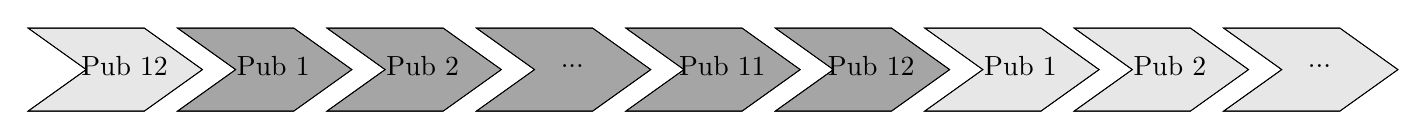
\begin{tikzpicture}
\pgftransformxscale{1.000000}
\pgftransformyscale{-1.000000}
\definecolor{dialinecolor}{rgb}{0.000000, 0.000000, 0.000000}
\pgfsetstrokecolor{dialinecolor}
\definecolor{dialinecolor}{rgb}{1.000000, 1.000000, 1.000000}
\pgfsetfillcolor{dialinecolor}
\pgfsetlinewidth{0.020000\du}
\pgfsetdash{}{0pt}
\pgfsetdash{}{0pt}
\pgfsetbuttcap
\pgfsetmiterjoin
\pgfsetlinewidth{0.020000\du}
\pgfsetbuttcap
\pgfsetmiterjoin
\pgfsetdash{}{0pt}
\definecolor{dialinecolor}{rgb}{0.905882, 0.905882, 0.905882}
\pgfsetfillcolor{dialinecolor}
\fill (9.200000\du,6.000000\du)--(12.000000\du,6.000000\du)--(13.400000\du,7.000000\du)--(12.000000\du,8.000000\du)--(9.200000\du,8.000000\du)--(10.600000\du,7.000000\du)--cycle;
\definecolor{dialinecolor}{rgb}{0.000000, 0.000000, 0.000000}
\pgfsetstrokecolor{dialinecolor}
\draw (9.200000\du,6.000000\du)--(12.000000\du,6.000000\du)--(13.400000\du,7.000000\du)--(12.000000\du,8.000000\du)--(9.200000\du,8.000000\du)--(10.600000\du,7.000000\du)--cycle;
\pgfsetbuttcap
\pgfsetmiterjoin
\pgfsetdash{}{0pt}
\definecolor{dialinecolor}{rgb}{0.000000, 0.000000, 0.000000}
\pgfsetstrokecolor{dialinecolor}
\draw (9.200000\du,6.000000\du)--(12.000000\du,6.000000\du)--(13.400000\du,7.000000\du)--(12.000000\du,8.000000\du)--(9.200000\du,8.000000\du)--(10.600000\du,7.000000\du)--cycle;
\pgfsetlinewidth{0.020000\du}
\pgfsetdash{}{0pt}
\pgfsetdash{}{0pt}
\pgfsetbuttcap
\pgfsetmiterjoin
\pgfsetlinewidth{0.020000\du}
\pgfsetbuttcap
\pgfsetmiterjoin
\pgfsetdash{}{0pt}
\definecolor{dialinecolor}{rgb}{0.647059, 0.647059, 0.647059}
\pgfsetfillcolor{dialinecolor}
\fill (12.800000\du,6.000000\du)--(15.600000\du,6.000000\du)--(17.000000\du,7.000000\du)--(15.600000\du,8.000000\du)--(12.800000\du,8.000000\du)--(14.200000\du,7.000000\du)--cycle;
\definecolor{dialinecolor}{rgb}{0.000000, 0.000000, 0.000000}
\pgfsetstrokecolor{dialinecolor}
\draw (12.800000\du,6.000000\du)--(15.600000\du,6.000000\du)--(17.000000\du,7.000000\du)--(15.600000\du,8.000000\du)--(12.800000\du,8.000000\du)--(14.200000\du,7.000000\du)--cycle;
\pgfsetbuttcap
\pgfsetmiterjoin
\pgfsetdash{}{0pt}
\definecolor{dialinecolor}{rgb}{0.000000, 0.000000, 0.000000}
\pgfsetstrokecolor{dialinecolor}
\draw (12.800000\du,6.000000\du)--(15.600000\du,6.000000\du)--(17.000000\du,7.000000\du)--(15.600000\du,8.000000\du)--(12.800000\du,8.000000\du)--(14.200000\du,7.000000\du)--cycle;
\pgfsetlinewidth{0.020000\du}
\pgfsetdash{}{0pt}
\pgfsetdash{}{0pt}
\pgfsetbuttcap
\pgfsetmiterjoin
\pgfsetlinewidth{0.020000\du}
\pgfsetbuttcap
\pgfsetmiterjoin
\pgfsetdash{}{0pt}
\definecolor{dialinecolor}{rgb}{0.647059, 0.647059, 0.647059}
\pgfsetfillcolor{dialinecolor}
\fill (16.400000\du,6.000000\du)--(19.200000\du,6.000000\du)--(20.600000\du,7.000000\du)--(19.200000\du,8.000000\du)--(16.400000\du,8.000000\du)--(17.800000\du,7.000000\du)--cycle;
\definecolor{dialinecolor}{rgb}{0.000000, 0.000000, 0.000000}
\pgfsetstrokecolor{dialinecolor}
\draw (16.400000\du,6.000000\du)--(19.200000\du,6.000000\du)--(20.600000\du,7.000000\du)--(19.200000\du,8.000000\du)--(16.400000\du,8.000000\du)--(17.800000\du,7.000000\du)--cycle;
\pgfsetbuttcap
\pgfsetmiterjoin
\pgfsetdash{}{0pt}
\definecolor{dialinecolor}{rgb}{0.000000, 0.000000, 0.000000}
\pgfsetstrokecolor{dialinecolor}
\draw (16.400000\du,6.000000\du)--(19.200000\du,6.000000\du)--(20.600000\du,7.000000\du)--(19.200000\du,8.000000\du)--(16.400000\du,8.000000\du)--(17.800000\du,7.000000\du)--cycle;
\pgfsetlinewidth{0.020000\du}
\pgfsetdash{}{0pt}
\pgfsetdash{}{0pt}
\pgfsetbuttcap
\pgfsetmiterjoin
\pgfsetlinewidth{0.020000\du}
\pgfsetbuttcap
\pgfsetmiterjoin
\pgfsetdash{}{0pt}
\definecolor{dialinecolor}{rgb}{0.647059, 0.647059, 0.647059}
\pgfsetfillcolor{dialinecolor}
\fill (20.000000\du,6.000000\du)--(22.800000\du,6.000000\du)--(24.200000\du,7.000000\du)--(22.800000\du,8.000000\du)--(20.000000\du,8.000000\du)--(21.400000\du,7.000000\du)--cycle;
\definecolor{dialinecolor}{rgb}{0.000000, 0.000000, 0.000000}
\pgfsetstrokecolor{dialinecolor}
\draw (20.000000\du,6.000000\du)--(22.800000\du,6.000000\du)--(24.200000\du,7.000000\du)--(22.800000\du,8.000000\du)--(20.000000\du,8.000000\du)--(21.400000\du,7.000000\du)--cycle;
\pgfsetbuttcap
\pgfsetmiterjoin
\pgfsetdash{}{0pt}
\definecolor{dialinecolor}{rgb}{0.000000, 0.000000, 0.000000}
\pgfsetstrokecolor{dialinecolor}
\draw (20.000000\du,6.000000\du)--(22.800000\du,6.000000\du)--(24.200000\du,7.000000\du)--(22.800000\du,8.000000\du)--(20.000000\du,8.000000\du)--(21.400000\du,7.000000\du)--cycle;
\pgfsetlinewidth{0.020000\du}
\pgfsetdash{}{0pt}
\pgfsetdash{}{0pt}
\pgfsetbuttcap
\pgfsetmiterjoin
\pgfsetlinewidth{0.020000\du}
\pgfsetbuttcap
\pgfsetmiterjoin
\pgfsetdash{}{0pt}
\definecolor{dialinecolor}{rgb}{0.647059, 0.647059, 0.647059}
\pgfsetfillcolor{dialinecolor}
\fill (23.600000\du,6.000000\du)--(26.400000\du,6.000000\du)--(27.800000\du,7.000000\du)--(26.400000\du,8.000000\du)--(23.600000\du,8.000000\du)--(25.000000\du,7.000000\du)--cycle;
\definecolor{dialinecolor}{rgb}{0.000000, 0.000000, 0.000000}
\pgfsetstrokecolor{dialinecolor}
\draw (23.600000\du,6.000000\du)--(26.400000\du,6.000000\du)--(27.800000\du,7.000000\du)--(26.400000\du,8.000000\du)--(23.600000\du,8.000000\du)--(25.000000\du,7.000000\du)--cycle;
\pgfsetbuttcap
\pgfsetmiterjoin
\pgfsetdash{}{0pt}
\definecolor{dialinecolor}{rgb}{0.000000, 0.000000, 0.000000}
\pgfsetstrokecolor{dialinecolor}
\draw (23.600000\du,6.000000\du)--(26.400000\du,6.000000\du)--(27.800000\du,7.000000\du)--(26.400000\du,8.000000\du)--(23.600000\du,8.000000\du)--(25.000000\du,7.000000\du)--cycle;
\pgfsetlinewidth{0.020000\du}
\pgfsetdash{}{0pt}
\pgfsetdash{}{0pt}
\pgfsetbuttcap
\pgfsetmiterjoin
\pgfsetlinewidth{0.020000\du}
\pgfsetbuttcap
\pgfsetmiterjoin
\pgfsetdash{}{0pt}
\definecolor{dialinecolor}{rgb}{0.647059, 0.647059, 0.647059}
\pgfsetfillcolor{dialinecolor}
\fill (27.200000\du,6.000000\du)--(30.000000\du,6.000000\du)--(31.400000\du,7.000000\du)--(30.000000\du,8.000000\du)--(27.200000\du,8.000000\du)--(28.600000\du,7.000000\du)--cycle;
\definecolor{dialinecolor}{rgb}{0.000000, 0.000000, 0.000000}
\pgfsetstrokecolor{dialinecolor}
\draw (27.200000\du,6.000000\du)--(30.000000\du,6.000000\du)--(31.400000\du,7.000000\du)--(30.000000\du,8.000000\du)--(27.200000\du,8.000000\du)--(28.600000\du,7.000000\du)--cycle;
\pgfsetbuttcap
\pgfsetmiterjoin
\pgfsetdash{}{0pt}
\definecolor{dialinecolor}{rgb}{0.000000, 0.000000, 0.000000}
\pgfsetstrokecolor{dialinecolor}
\draw (27.200000\du,6.000000\du)--(30.000000\du,6.000000\du)--(31.400000\du,7.000000\du)--(30.000000\du,8.000000\du)--(27.200000\du,8.000000\du)--(28.600000\du,7.000000\du)--cycle;
\pgfsetlinewidth{0.020000\du}
\pgfsetdash{}{0pt}
\pgfsetdash{}{0pt}
\pgfsetbuttcap
\pgfsetmiterjoin
\pgfsetlinewidth{0.020000\du}
\pgfsetbuttcap
\pgfsetmiterjoin
\pgfsetdash{}{0pt}
\definecolor{dialinecolor}{rgb}{0.905882, 0.905882, 0.905882}
\pgfsetfillcolor{dialinecolor}
\fill (30.800000\du,6.000000\du)--(33.600000\du,6.000000\du)--(35.000000\du,7.000000\du)--(33.600000\du,8.000000\du)--(30.800000\du,8.000000\du)--(32.200000\du,7.000000\du)--cycle;
\definecolor{dialinecolor}{rgb}{0.000000, 0.000000, 0.000000}
\pgfsetstrokecolor{dialinecolor}
\draw (30.800000\du,6.000000\du)--(33.600000\du,6.000000\du)--(35.000000\du,7.000000\du)--(33.600000\du,8.000000\du)--(30.800000\du,8.000000\du)--(32.200000\du,7.000000\du)--cycle;
\pgfsetbuttcap
\pgfsetmiterjoin
\pgfsetdash{}{0pt}
\definecolor{dialinecolor}{rgb}{0.000000, 0.000000, 0.000000}
\pgfsetstrokecolor{dialinecolor}
\draw (30.800000\du,6.000000\du)--(33.600000\du,6.000000\du)--(35.000000\du,7.000000\du)--(33.600000\du,8.000000\du)--(30.800000\du,8.000000\du)--(32.200000\du,7.000000\du)--cycle;
\pgfsetlinewidth{0.020000\du}
\pgfsetdash{}{0pt}
\pgfsetdash{}{0pt}
\pgfsetbuttcap
\pgfsetmiterjoin
\pgfsetlinewidth{0.020000\du}
\pgfsetbuttcap
\pgfsetmiterjoin
\pgfsetdash{}{0pt}
\definecolor{dialinecolor}{rgb}{0.905882, 0.905882, 0.905882}
\pgfsetfillcolor{dialinecolor}
\fill (34.400000\du,6.000000\du)--(37.200000\du,6.000000\du)--(38.600000\du,7.000000\du)--(37.200000\du,8.000000\du)--(34.400000\du,8.000000\du)--(35.800000\du,7.000000\du)--cycle;
\definecolor{dialinecolor}{rgb}{0.000000, 0.000000, 0.000000}
\pgfsetstrokecolor{dialinecolor}
\draw (34.400000\du,6.000000\du)--(37.200000\du,6.000000\du)--(38.600000\du,7.000000\du)--(37.200000\du,8.000000\du)--(34.400000\du,8.000000\du)--(35.800000\du,7.000000\du)--cycle;
\pgfsetbuttcap
\pgfsetmiterjoin
\pgfsetdash{}{0pt}
\definecolor{dialinecolor}{rgb}{0.000000, 0.000000, 0.000000}
\pgfsetstrokecolor{dialinecolor}
\draw (34.400000\du,6.000000\du)--(37.200000\du,6.000000\du)--(38.600000\du,7.000000\du)--(37.200000\du,8.000000\du)--(34.400000\du,8.000000\du)--(35.800000\du,7.000000\du)--cycle;
% setfont left to latex
\definecolor{dialinecolor}{rgb}{0.000000, 0.000000, 0.000000}
\pgfsetstrokecolor{dialinecolor}
\node[anchor=west] at (10.250000\du,6.917500\du){Pub 12};
% setfont left to latex
\definecolor{dialinecolor}{rgb}{0.000000, 0.000000, 0.000000}
\pgfsetstrokecolor{dialinecolor}
\node[anchor=west] at (14.000000\du,6.917500\du){Pub 1};
% setfont left to latex
\definecolor{dialinecolor}{rgb}{0.000000, 0.000000, 0.000000}
\pgfsetstrokecolor{dialinecolor}
\node[anchor=west] at (17.600000\du,6.912562\du){Pub 2};
% setfont left to latex
\definecolor{dialinecolor}{rgb}{0.000000, 0.000000, 0.000000}
\pgfsetstrokecolor{dialinecolor}
\node[anchor=west] at (21.800000\du,6.917500\du){    ...};
% setfont left to latex
\definecolor{dialinecolor}{rgb}{0.000000, 0.000000, 0.000000}
\pgfsetstrokecolor{dialinecolor}
\node[anchor=west] at (24.650000\du,6.917500\du){Pub 11};
% setfont left to latex
\definecolor{dialinecolor}{rgb}{0.000000, 0.000000, 0.000000}
\pgfsetstrokecolor{dialinecolor}
\node[anchor=west] at (28.237500\du,6.917500\du){Pub 12};
% setfont left to latex
\definecolor{dialinecolor}{rgb}{0.000000, 0.000000, 0.000000}
\pgfsetstrokecolor{dialinecolor}
\node[anchor=west] at (32.000000\du,6.912562\du){Pub 1};
% setfont left to latex
\definecolor{dialinecolor}{rgb}{0.000000, 0.000000, 0.000000}
\pgfsetstrokecolor{dialinecolor}
\node[anchor=west] at (35.600000\du,6.912562\du){Pub 2};
\pgfsetlinewidth{0.020000\du}
\pgfsetdash{}{0pt}
\pgfsetdash{}{0pt}
\pgfsetbuttcap
\pgfsetmiterjoin
\pgfsetlinewidth{0.020000\du}
\pgfsetbuttcap
\pgfsetmiterjoin
\pgfsetdash{}{0pt}
\definecolor{dialinecolor}{rgb}{0.905882, 0.905882, 0.905882}
\pgfsetfillcolor{dialinecolor}
\fill (38.000000\du,6.000000\du)--(40.800000\du,6.000000\du)--(42.200000\du,7.000000\du)--(40.800000\du,8.000000\du)--(38.000000\du,8.000000\du)--(39.400000\du,7.000000\du)--cycle;
\definecolor{dialinecolor}{rgb}{0.000000, 0.000000, 0.000000}
\pgfsetstrokecolor{dialinecolor}
\draw (38.000000\du,6.000000\du)--(40.800000\du,6.000000\du)--(42.200000\du,7.000000\du)--(40.800000\du,8.000000\du)--(38.000000\du,8.000000\du)--(39.400000\du,7.000000\du)--cycle;
\pgfsetbuttcap
\pgfsetmiterjoin
\pgfsetdash{}{0pt}
\definecolor{dialinecolor}{rgb}{0.000000, 0.000000, 0.000000}
\pgfsetstrokecolor{dialinecolor}
\draw (38.000000\du,6.000000\du)--(40.800000\du,6.000000\du)--(42.200000\du,7.000000\du)--(40.800000\du,8.000000\du)--(38.000000\du,8.000000\du)--(39.400000\du,7.000000\du)--cycle;
% setfont left to latex
\definecolor{dialinecolor}{rgb}{0.000000, 0.000000, 0.000000}
\pgfsetstrokecolor{dialinecolor}
\node[anchor=west] at (39.800000\du,6.917500\du){   ...};
\end{tikzpicture}

	  \end{center}
	  \caption{Roulement de la publicité}
	  \label{fig:roulementPub}
  \end{figure}

  La démarche de monétisation despaces publicitaires débutera lorsqu'un nombre 
  d'utilisateurs suffisant sera atteint (environ 3000). Ce nombre sera calculé
  en fonction des téléchargemtents initiés depuis noter site internet. Les prix de
  vente des espaces publicitaires sont fixés par rapport à la concurrence. Bien
  qu'indirecte, elle touche le même volume d'entreprise. Le prix d'une pleine plage
  de publicité dans un magasine spécialisé est d'environ 10k\euro{}/mois. Il est 
  prévu dans un premier temps d'adopter une politique de pénétration de marché et de
  faire une offre de lancement à 5k\euro{}/mois pendant 6 mois pour 5 minutes
  d'affichage par heure. Ce pric prévoit une durée durée d'affiche de 5 minutes par heure.
  Si l'annonceur désire une plus grande visibilité, il pourra acheter des espaces
  d'affichafe plus grands. Aussi, un tarif dégressif sera appliqué (cf. tableau
  \ref{tab:tarifsPub}).
  \begin{table}[H]
	  \centering
	  \rowcolors{2}{grisclair}{grisfonce}
	  \begin{tabular}{>{\begin{bf}} c <{\end{bf}}|c|c}
		  \hline
		  Temps d'affichage (min) & \textbf{Prix HT (\euro{})} &
				  \textbf{Prix HT par minute (\euro{})} \\
		  \hline
		  5  & 5 000  & 1 000 \\
		  10 & 9 200  & 920 \\
		  15 & 12 600 & 840 \\
		  20 & 15 200 & 760 \\
		  25 & 17 000 & 680 \\
		  30 & 18 000 & 600 \\
		  \hline
	  \end{tabular}
	  \caption{Tarifs des espaces publicitaires en fonction du temps d'affichage par heure}
	  \label{tab:tarifsPub}
  \end{table}

  Notre offre possédant des avantages non négligeables par rapport à la concurrence
  (interractivité, durée de visibilité, etc.) sera donc à terme plus chère. Il est
  prévu à moyen terme un objectif de 20 à 25k\euro{} par mois.\\

  Etant donné que notre force de vente réside dans le nombre d'urilisateurs de notre logiciel,
  la communication les visera exclusivement. pour ce faire , la communication s'éeffectuera
  par le biais d'un annuaire d'adresses mail, réalisé par nos soins, regroupant environ 6000
  entreprises du secteur. il est prévu de faire un campagne de communiaction par l'intermédiaire
  d'une vidéo de moins d'une minute. Cette vidéo sera hébergée sur Youtube. L'intérêt
  est double : donner une image dynamique de la société grâce à un support non convientionnel,
  et montrer tout le manel de fonctionnalités présentes dans notre produit. De plus un achat
  de mot-clé Google Adwords est envisagé.

  La distribution s'effectuera par la biais du site internet \url{www.klimasoft.fr}.
  Les visiteurs pourront télécharger gratuitement le logiciel.

